\documentclass[10pt,aspectratio=43]{beamer}
\usetheme{Berlin}

\usepackage{amsmath,bm,amsfonts,amssymb,enumerate,graphicx,animate,epsfig,bbm,calc,color,ifthen,capt-of,multimedia}
\usepackage{fancybox,xcolor,booktabs,colortbl}
\usepackage{physics}
\usepackage{../mycommand}%我惯用的命令,在本project中,存储在本文件的父文件夹
\graphicspath{{../figures/}}

\usefonttheme{professionalfonts}
\usepackage[UTF8,fontset=none,scheme=chinese]{ctex}
\setmainfont{Times}
\setsansfont{Arial}
\setmonofont{Consolas}
\setCJKmainfont{SimSun}[BoldFont=SimHei,ItalicFont=KaiTi]
\setCJKsansfont{SimHei}
\setCJKmonofont{Microsoft YaHei}
\usepackage{unicode-math}
\setmathfont{XITS Math}

\usecolortheme{sustech}
\definecolor{mygreen}{rgb}{0,0.6,0}
\definecolor{mymauve}{rgb}{0.58,0,0.82}
\definecolor{mygray}{gray}{.9}
\definecolor{mypink}{rgb}{.99,.91,.95}
\definecolor{mycyan}{cmyk}{.3,0,0,0}

\usepackage[ruled,linesnumbered]{algorithm2e}
\usepackage{verbatim,listings}
\lstset{ %
	backgroundcolor=\color{white},   % choose the background color
	basicstyle=\footnotesize\ttfamily,     % size of fonts used for the code
	columns=fullflexible,
	breaklines=true,                 % automatic line breaking only at whitespace
	captionpos=b,                    % sets the caption-position to bottom
	tabsize=4,
	commentstyle=\color{mygreen},    % comment style
	escapeinside={\%*}{*)},          % if you want to add LaTeX within your code
	keywordstyle=\color{blue},       % keyword style
	stringstyle=\color{mymauve}\ttfamily,     % string literal style
	numbers=left, 
	%	frame=single,
	rulesepcolor=\color{red!20!green!20!blue!20},
	% identifierstyle=\color{red},
	language=c
}

\setbeamertemplate{caption}[numbered]%添加图片的编号
\setbeamertemplate{sidebar right}{}%去掉默认添加的navigarion symbols
\setbeamercovered{transparent}%使未点出来的文字呈现透明,默认0.15透明度

\usepackage[backend=biber,bibstyle=gb7714-2015,citestyle=verbose]{biblatex}
\addbibresource{../reference.bib}

%题目,作者,学校,日期
\title{里德堡原子基态拓扑量子信息传输}
\subtitle{\fontsize{9pt}{14pt}\textbf{毕业论文开题报告}}
\author{答辩人:杨徵羽 \quad 指导教师:吴金雷}
\institute{哈尔滨工业大学(威海)理学院}
\date{\today}

%学校Logo
%\pgfdeclareimage[height=0.5cm]{sustech-logo}{sustech-logo.pdf}
%\logo{\pgfuseimage{sustech-logo}\hspace*{0.3cm}}

\AtBeginSection[]
{
	\begin{frame}<beamer>
	\frametitle{\textbf{目录}}
	\tableofcontents[currentsection]
\end{frame}
}
\beamerdefaultoverlayspecification{<+->}

\begin{document}

\frame{\titlepage}

\section[目录]{}   %目录
\begin{frame}{目录}
\tableofcontents
\end{frame}

\section{课题背景}
\begin{frame}{量子信息技术}
量子信息技术的优势
\begin{enumerate}
\item 研究真实世界演化:只有用量子计算机才能高效模拟量子世界\footcite{1999Simulating}%此处引用有bug???
\item 快速算法:如Grover搜索算法、Shor质因数分解算法
\item 量子隐形传态:一旦窃听就会暴露
\item ……
\end{enumerate}
当前的研究障碍
\begin{enumerate}
\item 硬件上,可用的量子比特数目和量子门操作保真度远远没有达到量子计算机要求
\item 软件上,能发挥量子计算优势的量子算法难以编写
\end{enumerate}
\end{frame}
\begin{frame}{量子比特与量子逻辑门}
单个量子比特:$ \ket{\psi}=\alpha\ket{0}+\beta\ket{1} $

多个量子比特:$ \ket{\psi}=\sum\alpha_{i_1\cdots i_n}\ket{i_1\cdots i_n},~i_1,\cdots,i_n=0,1 $

单量子比特门:如Hadamard门,Pauli-X门
\begin{figure}
\centering
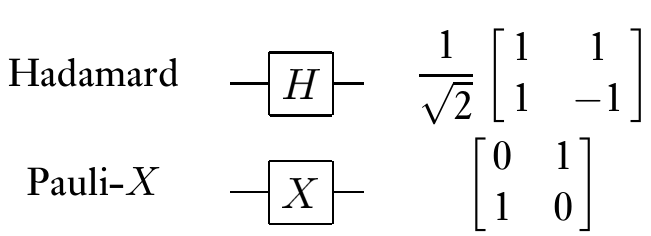
\includegraphics[scale=0.25]{gate1}
%\caption{}
\label{fig:gate1}
\end{figure}

多量子比特门:如Controlled-NOT门,SWAP门,Toffoli门
\begin{figure}
\centering
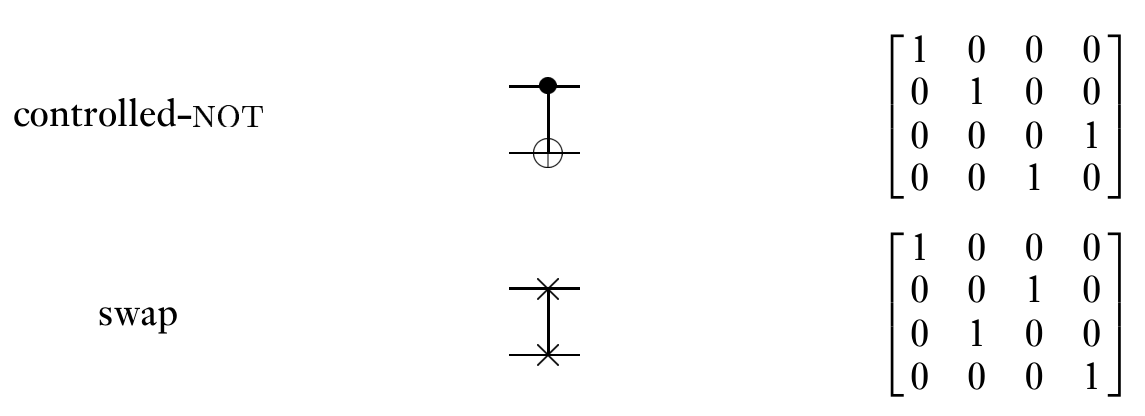
\includegraphics[scale=0.25]{gaten}
%\caption{}
\label{fig:gaten}
\end{figure}
\end{frame}

\begin{frame}{实现量子逻辑门的物理方法}
当前有潜力实现量子计算的物理平台有很多,如
\begin{enumerate}
\item 囚禁离子量子比特平台
\item 超导人造原子量子比特平台
\item 囚禁中性原子量子比特平台
\item 中性里德堡原子平台
\end{enumerate}
中性里德堡原子平台的优势
\begin{enumerate}
\item 完美全同、易于扩展、相干时间长
\item 具有良好的连通性,里德堡原子平台具有实现涉及超过两个原子的多量子比特门
\item 仅仅通过使用外部的控制场便可以实现对中性原子外部状态和内部状态的操纵
\end{enumerate}
\end{frame}

\begin{frame}{里德堡原子}
里德堡原子:处于主量子数$ n $很大的量子态的原子

里德堡相互作用:多个里德堡原子的相互作用
\begin{enumerate}
\item 两个原子,跃迁能量差相等:偶极-偶极相互作用,$ V\propto R^{-3} $
\item 两个原子,跃迁能量差不等:van der Vaals相互作用,$ V\propto R^{-6} $
\item 三个及以上原子:F\"orster共振相互作用
\end{enumerate}

\begin{figure}
\begin{minipage}{0.4\linewidth}
\centering
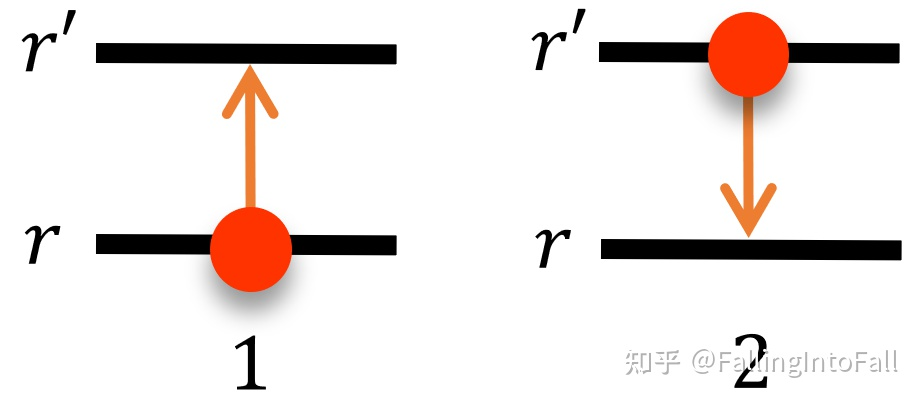
\includegraphics[width=\linewidth]{v-dd}
\caption{偶极-偶极相互作用}
\label{fig:v-dd}
\end{minipage}
\qquad
\begin{minipage}{0.4\linewidth}
\centering
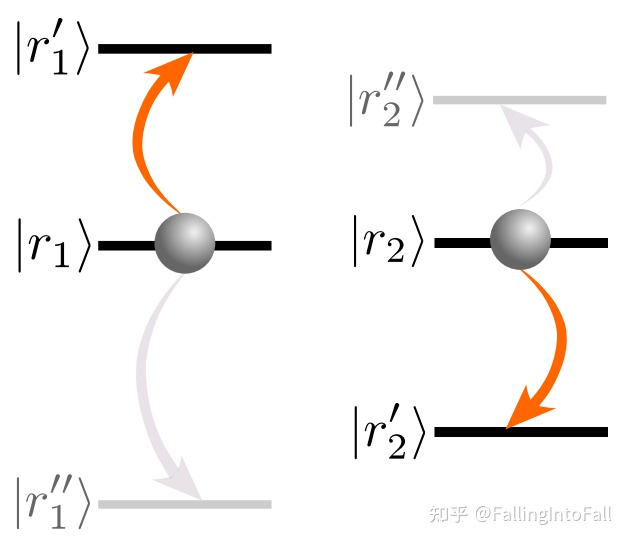
\includegraphics[width=0.8\linewidth]{v-vdw}
\caption{van der Vaals相互作用}
\label{fig:v-vdw}
\end{minipage}
\end{figure}

\end{frame}

\begin{frame}{研究里德堡原子系统的一般步骤}
\begin{enumerate}
\item 写出系统的哈密顿量
\item 选取适当的表象,对哈密顿量进行变换,从而化简
\item 取大失谐近似,求出系统的有效哈密顿量
\item 分析系统性质(最一般的方法是解薛定谔方程,但也可以直接从有效哈密顿量的各项系数中看出系统的性质)
\end{enumerate}
\end{frame}
\section{当前进展}
\begin{frame}{哈密顿量}
目前复现了\footcite{PhysRevA.105.032417}的一部分:两个Λ型原子与光场Raman相互作用
\begin{figure}
\centering
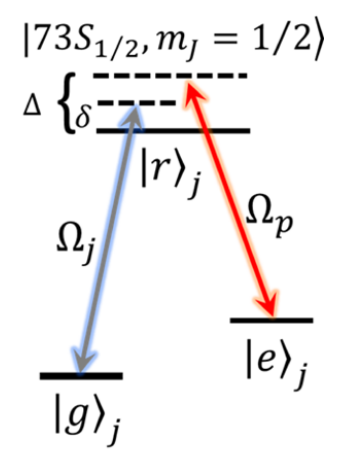
\includegraphics[height=0.5\textheight]{pra-energy-level}
\caption{能级示意图(只显示了其中一个原子)}
\label{fig:pra-energy-level}
\end{figure}
\end{frame}

\begin{frame}{哈密顿量}
在半经典理论中,单个原子与光场作用的哈密顿量为
\begin{equation}
H_j^\mathrm{S}=\hbar(\omega_g\ketbra{g}{g}_j+\omega_i\ketbra{r}{r}_j+\omega_e\ketbra{e}{e}_j+(\Omega_j\ketbra{g}{r}_j+\Omega_p\ketbra{e}{r}_j+\hc))
\end{equation}
变换到相互作用绘景,得
\begin{equation}\label{}
H_j^\mathrm{I}=\hbar(\mathrm{e}^{\mathrm{i}t\delta}\Omega_j\ketbra{g}{r}_j+\mathrm{e}^{\mathrm{i}t\Delta}\Omega_p\ketbra{e}{r}_j+\hc)
\end{equation}
其中$ \delta=\Omega-\omega_r+\omega_g,\Delta=\Omega_p-\omega_r+\omega_e
 $为失谐量,其量级满足
\begin{equation}
\Delta\gg\delta\sim\Omega_p\gg\Omega_j
\end{equation}
\end{frame}

\begin{frame}{哈密顿量}
故两个原子的与光场作用的哈密顿量为
\begin{multline}
H^\mathrm{I}=I_1\otimes H_2+H_1\otimes I_2\\
=\hbar(\Omega_1\mathrm{e}^{\mathrm{i}t\delta}\ketbra{gg}{rg}
+\Omega_1\mathrm{e}^{\mathrm{i}t\delta}\ketbra{ge}{re}
+\Omega_1\mathrm{e}^{\mathrm{i}t\delta}\ketbra{gr}{rr}\\
+\Omega_p\mathrm{e}^{\mathrm{i}t\Delta}\ketbra{eg}{rg}
+\Omega_p\mathrm{e}^{\mathrm{i}t\Delta}\ketbra{ee}{re}
+\Omega_p\mathrm{e}^{\mathrm{i}t\Delta}\ketbra{er}{rr}\\
+\Omega_2\mathrm{e}^{\mathrm{i}t\delta}\ketbra{gg}{gr}
+\Omega_2\mathrm{e}^{\mathrm{i}t\delta}\ketbra{eg}{er}
+\Omega_2\mathrm{e}^{\mathrm{i}t\delta}\ketbra{rg}{rr}\\
+\Omega_p\mathrm{e}^{\mathrm{i}t\Delta}\ketbra{ge}{gr}
+\Omega_p\mathrm{e}^{\mathrm{i}t\Delta}\ketbra{ee}{er}
+\Omega_p\mathrm{e}^{\mathrm{i}t\Delta}\ketbra{re}{rr}
+\hc)
\end{multline}
考虑到van der Vaals相互作用,并采用旋波近似,经一系列分析,上式可简化为
\begin{equation}
H^{\mathrm{II}}=\hbar(\Omega_1\eit{\delta}\ketbra{ge}{re}
+\Omega_p\ketbra{er}{rr}
+\Omega_2\eit{\delta}\ketbra{eg}{er}
+\Omega_p\ketbra{re}{rr}+\hc)
\end{equation}

\end{frame}
\begin{frame}{表象变换}
将$ H^{\mathrm{II}} $中的不含时项对角化得
{\small\begin{equation}
\begin{gathered}
E_+=\sqrt{2}\hbar\Omega_p,\quad\ket{\psi_+}=\frac{1}{2}\ket{er}+\frac{1}{\sqrt{2}}\ket{rr}+\frac{1}{2}\ket{re},\\
E_0=0,\quad\ket{\psi_0}=\frac{1}{\sqrt{2}}\ket{er}-\frac{1}{\sqrt{2}}\ket{re},\\
E_-=-\sqrt{2}\hbar\Omega_p,\quad\ket{\psi_-}=\frac{1}{2}\ket{er}-\frac{1}{\sqrt{2}}\ket{rr}+\frac{1}{2}\ket{re}
\end{gathered}
\end{equation}}
将其本征态$ \ket{\psi_+},\ket{\psi_0},\ket{\psi_-} $作为新的基,再进行相互作用绘景变换,得到最终哈密顿量的形式为
{\small\begin{multline}\label{hiii}
H^{\mathrm{III}}=\hbar\Omega\Bigg(\ket{ge}\Bigg(\frac{1}{2}\bra{\psi_+}\mathrm{e}^{\mathrm{i}t(\delta-\sqrt{2}\Omega_p)}-\frac{1}{\sqrt{2}}\bra{\psi_0}\eit{\delta}+\frac{1}{2}\bra{\psi_-}\eit{(\delta+\sqrt{2}\Omega_p)}\Bigg)\\
+\ket{eg}\Bigg(\frac{1}{2}\bra{\psi_+}\mathrm{e}^{\mathrm{i}t(\delta-\sqrt{2}\Omega_p)}+\frac{1}{\sqrt{2}}\bra{\psi_0}\eit{\delta}+\frac{1}{2}\bra{\psi_-}\eit{(\delta+\sqrt{2}\Omega_p)}\Bigg)\Bigg)+\hc
\end{multline}}
\end{frame}
\begin{frame}{有效哈密顿量}
利用论文\footcite{James2007EffectiveHT}的方法,可得有效哈密顿量为
{\footnotesize\begin{multline}
H_{\eff}=\hbar\Omega^2\Bigg(\frac{1}{\delta-\sqrt{2}\Omega_p}\left(-\frac{1}{4}\ketbra{eg}{ge}\right)+\frac{1}{\delta}\left(-\frac{1}{2}\ketbra{eg}{ge}\right)\\
+\frac{1}{\delta+\sqrt{2}\Omega_p}\left(-\frac{1}{4}\ketbra{eg}{ge}\right)+\hc
+\frac{1}{\delta-\sqrt{2}\Omega_p}\left(\frac{1}{4}(-\ketbra{ge}{ge}-\ketbra{eg}{eg})\right)\\
+\frac{1}{\delta}\left(\frac{1}{2}(-\ketbra{ge}{ge}-\ketbra{eg}{eg})\right)
+\frac{1}{\delta+\sqrt{2}\Omega_p}\left(\frac{1}{4}(-\ketbra{ge}{ge}-\ketbra{eg}{eg})\right)\Bigg)
\end{multline}}
其中耦合系数($ \ketbra{eg}{ge} $项的系数)为
{\small\begin{equation}
J_{12}=\frac{\Omega^2}{4}\Bigg(\frac{1}{\delta-\sqrt{2}\Omega_p}-\frac{2}{\delta}+\frac{1}{\delta+\sqrt{2}\Omega_p}\Bigg)=\frac{\Omega^2\Omega_p^2}{\delta^3-2\delta\Omega_p^2}
\end{equation}}
这说明系统是一个SWAP门,$ J_{12} $反映了量子门的开关速率
\end{frame}
\section{未来计划}
\begin{frame}{快速SWAP门}
\begin{multline*}
H^{\mathrm{III}}=\hbar\Omega\Bigg(\ket{ge}\Bigg(\frac{1}{2}\bra{\psi_+}\mathrm{e}^{\mathrm{i}t(\delta-\sqrt{2}\Omega_p)}-\frac{1}{\sqrt{2}}\bra{\psi_0}\eit{\delta}+\frac{1}{2}\bra{\psi_-}\eit{(\delta+\sqrt{2}\Omega_p)}\Bigg)\\
+\ket{eg}\Bigg(\frac{1}{2}\bra{\psi_+}\mathrm{e}^{\mathrm{i}t(\delta-\sqrt{2}\Omega_p)}+\frac{1}{\sqrt{2}}\bra{\psi_0}\eit{\delta}+\frac{1}{2}\bra{\psi_-}\eit{(\delta+\sqrt{2}\Omega_p)}\Bigg)\Bigg)+\hc
\end{multline*}
在式 \eqref{hiii} 中,令$ \delta-\sqrt{2}\omega_p=0 $,则含相位$ \delta $和$ \delta-\sqrt{2}\omega_p $的项均可忽略。此时可构建具有$ \ket{eg} $、$ \ket{ge} $、$ \psi_+ $三个能级的系统,而$ J_{12} $数量级有望减小,从而实现更快速的SWAP门。
\end{frame}
\begin{frame}{拓扑量子信息传输}
将2个原子推广成一列原子,此时有望实现量子态从最左的原子传到最右边,即实现拓扑量子信息传输。
\begin{figure}
\centering
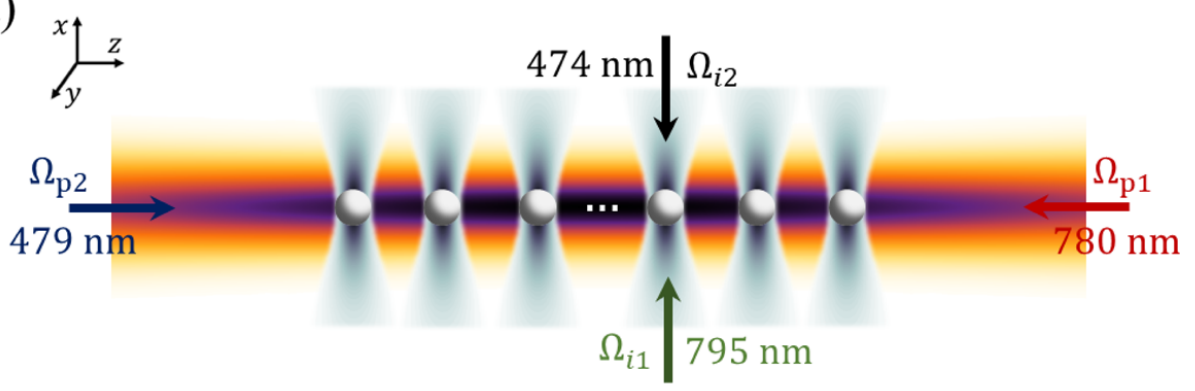
\includegraphics[width=0.7\linewidth]{pra-energy-level-n}
\caption{一维原子链}
\label{fig:pra-energy-level-n}
\end{figure}

\end{frame}

% 现在在每页脚注加参考文献,故不需要专门放一页参考文献
%\begin{frame}{参考文献}
%\printbibliography
%\end{frame}

\begin{frame}{}
\begin{center}
\begin{minipage}{1\textwidth}
\setbeamercolor{mybox}{fg=white, bg=black!50!blue}
\begin{beamercolorbox}[wd=0.70\textwidth, rounded=true, shadow=true]{mybox}
\LARGE \centering 请各位老师批评指正
\end{beamercolorbox}
\end{minipage}
\end{center}
\end{frame}

\end{document}
